% Chapter 2 - Background

\glsresetall % reset the glossary to expand acronyms again
\chapter[Literature Review]{Literature Review}\label{ch:LitReview}
\index{Literature Review}

%What to expact in this chapter

This chapter provides a comprehensive evaluation of literature relevant to the research topic. It begins with an introductory section outlining the motivation for the study, focusing on the need to further investigate mobile app development for digitising and storing ECG paper records. A brief overview of the theory behind ECG signal formation follows, providing the foundation for understanding its digitisation. 

The review then adopts a funnel approach: first examining existing methods of ECG record digitisation, then evaluating the potential of mobile applications for this purpose through image capture, and finally considering techniques for extracting ECG waveforms from images. The chapter concludes with a summary of key findings, identifying gaps in current research and setting the stage for the methodology that follows.

%----------------------------------------------------------------------------------------------

\section{Introduction}

The electrocardiogram (ECG) has been a fundamental tool in medicine since 1901 \cite{MartinezPerez2013MobileAppsCardiology}. Over the years, a vast number of ECG paper records have been produced. Consequently, researchers have devised methods to digitise these records in order to ensure long-term preservation, improve accessibility, and facilitate future evaluation and diagnosis. It is therefore important to investigate and assess these methods to understand their respective strengths and limitations.

With the growing use of mobile applications in healthcare \cite{Steinhubl2013CanMHealth}, new opportunities for ECG digitisation have emerged. This enables investigation into whether ECG images captured with mobile devices can be effectively processed for digitisation.

%----------------------------------------------------------------------------------------------

\section{ECG Fundamentals} \label{sec: ECG_Fund}
% the problem with this section is that it doesn't add points to delebarate over - how advantageous or disadvantageous or how the results sway the decsions

Electrocardiogram signals show how the path of the \gls{depolarization wave} - the flow of a group of positive electric charges - moves during each heartbeat \cite{osmosisECGbasics2025}. Hearts have natural pacemakers that initiate electric signals that cause atrial and ventricular contraction \cite{myhealthSAnode2024}. Electrocardiograms are built to sense these natural signals and convert them into useful information that portray the heart's condition.

\subsection{ECG Signal Generation}

The electric activity of the heart is governed by the sinoatrial (SA) and atrioventricular (AV) nodes. The SA node initialises the impulses and the AV node introduces delays to their delivery to co-ordinate between arterial and ventricular contractions for optimum heart functionality \cite{myhealthSAnode2024}.

As the positive charges move through the heart's muscles, their negative resting state changes to a positive active state. This change in charge of the internal muscles affects a change to the external charge surrounding it \cite{osmosisECGbasics2025}. This creates the potential difference measured by the electrocardiogram electrodes. If detected it is noted as a deflection on the ECG waveform. The bigger the potential difference, the larger the deflection \cite{osmosisECGbasics2025}.

(image explaining or showing ECG deflections - so they know what to look for in the actual trace)

\subsection{ECG Waveform Formation}

An ECG signal consists of five deflections that together form the PQRST complex, representing a single heartbeat and the complete cycle of myocardial contraction and relaxation \cite{AlGhatrif2012}.

The P wave reflects atrial depolarisation, initiating atrial contraction. It is typically a low-amplitude, gently sloped deflection due to the slower propagation of the depolarisation wave through atrial myocardial cells \cite{OReilly2023ModelDrivenAO}. The QRS complex corresponds to ventricular depolarisation and the onset of ventricular contraction, with the R wave being the largest positive deflection \cite{Prima2018PolyanilineAN}. The T wave represents ventricular repolarisation, preparing the ventricles for the next cardiac cycle \cite{Prima2018PolyanilineAN}.

\begin{figure}[H]
    \centering
    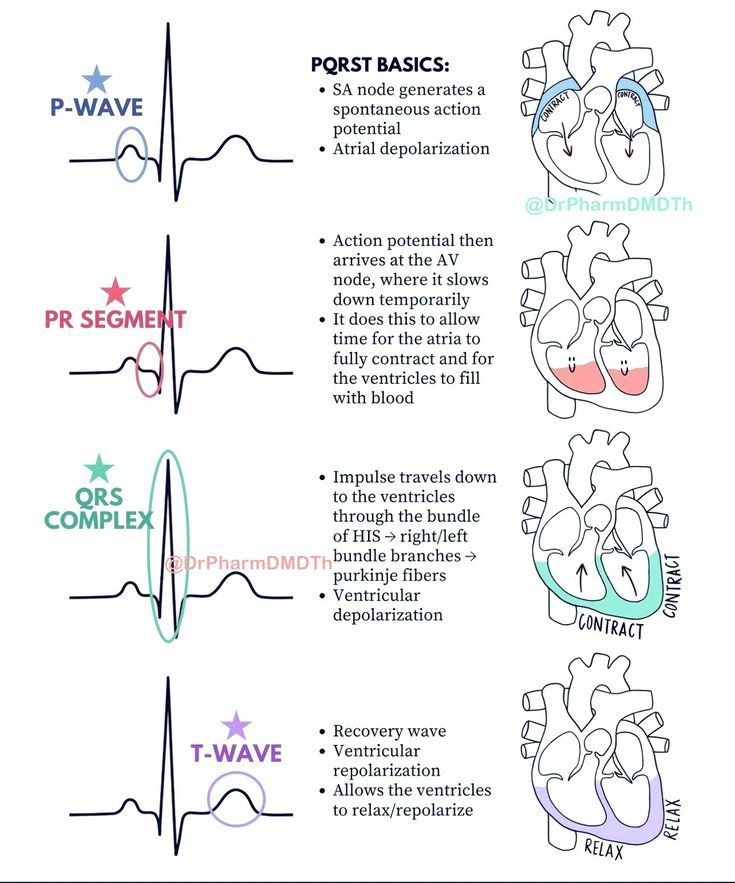
\includegraphics[width=0.4\textwidth]{3_Chapters/2_Chapter_LiteratureReview/Figures/PQRST_complex.jpg}
    \caption{Placeholder for ECG diagram}
    \label{fig:ECG_Waveform}
\end{figure}

The timing and amplitude of the PQRST wave are essential for patient health analysis \cite{Sinha2023SemiSupervisedCD}. Significant signal loss in the digisation process would thus render the ECG useless for diagnostic purposes.

\subsection{ECG leads}

The direction of this wave is dependent on the leads. The leads are defined by the electrodes used. In a 12-lead ECG, there are 10 electrodes used to measure the heart's activity from different angle and planes. Each lead provides different and vital information about arrhythmias and myocardial infarction (heart attacks). 

There are the limb electrodes places by the left arm and leg and the right arm. Measurements between two of them, with the third being a reference, creates the I, II, and III dipoles leads. When a fourth electrode known as the reference or zero electrode is introduced, the augmented leads are created. This is a measurement from one of the limb electrodes to the reference electrodes. This creates one of the unilateral leads. 

In 1934, it was noted that there were areas in the heart that needed to be measured to better detect myocardial infarctions. This gave birth to the precordial leads through the use of six electrodes placed around the precordial (chest area about and around the heart). 

These make up the 12 leads that illustrate the different waveform patterns seen in the electrocardiogram trace. They are used to section the ECG into 12 important regions which can be segmented and analysed further. \cite{AlGhatrif2012}

%----------------------------------------------------------------------------------------------

\section{Traditional ECG Digitisation Methods}

Digitisation of ECG paper records has been an area of interest for decades, with various methods developed to convert analog ECG signals into digital formats. This section reviews traditional digitisation techniques, highlighting their methodologies, advantages, and limitations.

Flatbed scanning and manual transcription have been attempted. Advantage: Simple and low-cost. Disadvantage: Manual methods are time-consuming and scanning introduces distortions and noise requiring post-processing \cite{Mishra2021}.

Scanning with morphological filtering was widely used. \textbf{Advantage}: Controlled scan environment ensures consistent image quality. Produces clean signals with high-resolution scans. \textbf{Disadvantage}: Not portable compared to smartphones, At lower resolution (300 dpi), characters cannot be removed effectively and waveform loss occur. \cite{Tun2017}.

Standard paper ECGs use a grid with scaling of 25 mm/s (time) and 10 mm/mV (voltage), arranged in a 3x4 lead display %digitising ECG image.

Factors like paper degradation and print resolution can introduce noise, affecting digitization accuracy \cite{LI2020104077}.

%-------------------------------------------------------

\section{Smartphone-based ECG Capturing}

Smartphones enable easy ECG capture with modern cameras. Advantage: High accessibility and does not require hospital scanners. Disadvantage: Image quality highly dependent on lighting, perspective, and shadows \cite{Mishra2021}.

Smartphones offer high-resolution cameras and processing power, making them viable for ECG capture. However, general document scanning apps lack ECG-specific features, such as grid removal and signal enhancement. Existing ECG apps often fail to handle highly noisy or binary scans effectively \cite{LI2020104077}.

%-------------------------------------------------------

\section{ECG Digitisation from Images}
% This is where we get into the details of the methods that have been used and developed for ECG digitisation from paper

\subsection{Image Pre-processing}

For camera images, the following is performed: RGB-channel splitting, dilation to suppress dark shadows, median blurring, and normalization to reduce salt-and-pepper noise; enabling field capture and materially improves thresholding and downstream extraction, but it still struggles with non-uniform illumination and requires careful text removal to avoid signal damage where labels overlap the trace. \cite{Mishra2021}

\subsubsection{De-warping and Perspective Correction}

\textbf{Hough Transform–Based Rectification:} The Hough Transform exploits the regular grid structure typically present in ECG reports. It detects straight lines—whether slanted, vertical, or horizontal—and uses their intersections to classify geometric shapes. Once identified, geometric rectification is applied by mapping these intersections (corners) to an ideal square lattice. This process expands or contracts distorted lines so that rhombi and parallelograms are reformed into rectangles. Such an approach effectively aligns warped grids, although its performance is sensitive to scan quality and noise in the image \cite{LI2020104077}.

\textbf{Geometric Rectification:} In addition to Hough-based detection, geometric rectification is widely used to correct perspective distortions introduced during image capture. For ECGs, perspective skew can significantly affect the readability of waveforms. By applying geometric transformations, images are realigned to restore proportionality between the waveform and grid axes. While this method is often combined with Hough detection for corner localization, its accuracy is dependent on reliable feature extraction and the absence of severe scanning artifacts.

%-------------------------------------------------------

\subsubsection{Noise Reduction} 

Noise reduction is a crucial preprocessing step in ECG image analysis, as various methods offer trade-offs between suppressing artifacts and preserving clinically important waveform features. These approaches range from traditional filtering techniques to deep learning models, each with distinct advantages and limitations.

\textbf{Median Filtering:} Median filtering replaces each pixel with the median of its local neighborhood. It is particularly effective at removing salt-and-pepper noise and is computationally efficient. However, it has limited effectiveness against structured noise such as grid lines. Moreover, median filtering can blur sharp ECG features, most notably the QRS complexes, thereby reducing diagnostic accuracy \cite{LI2020104077}.

\textbf{Adaptive Filtering:} Adaptive filtering modifies smoothing strength based on local noise levels, enabling better edge preservation compared to uniform filters. While this method reduces over-smoothing and retains more waveform detail, it continues to struggle with grid-line interference. Studies indicate that adaptive filters alone are insufficient for ECG applications and typically require additional post-processing to achieve acceptable results.

\textbf{Wavelet Denoising:} Wavelet-based approaches employ frequency-domain thresholding to suppress noise, and are effective for reducing Gaussian noise. However, they risk distorting high-frequency ECG components, including the QRS complex. The success of wavelet denoising is highly dependent on threshold selection, where overly aggressive thresholds may inadvertently remove clinically significant features \cite{LI2020104077}.

\textbf{Grayscale Scanning Pathway:} As an alternative approach grayscale contrast adjustment (imadjust) can be used to enhance the visibility of waveforms before thresholding. This is followed by morphological background estimation and subtraction. The technique is advantageous because it requires only a few parameters and executes quickly. However, it often leaves residual artifacts that must be corrected later through region-based segmentation. Furthermore, high-resolution scanning (around 600 dpi) is necessary to avoid jagged or discontinuous waveform outputs \cite{Tun2017AnalysisOC}.

\textbf{Deep Learning Approaches:} Recent advances include the use of U-Net architectures with ResNet blocks and attention mechanisms. In Li et al.’s evaluation, this method achieved a DICE similarity coefficient of 0.85 and a Pearson correlation of less than 0.9. The DICE coefficient measures the overlap between predicted and ground-truth segmentations, making it a critical index for assessing segmentation accuracy in biomedical imaging. This approach automatically handles diverse noise types without manual parameter tuning and outperforms traditional methods. However, it requires large annotated datasets for training, demands high computational resources, and still struggles with preserving sharp QRS transitions—an essential factor for accurate interval measurements.

Overall, all methods face the fundamental trade-off between noise suppression and feature preservation. Traditional techniques such as median, adaptive, and wavelet filtering are computationally efficient and straightforward to implement but struggle with structured noise and tend to degrade sharp ECG features. Deep learning methods demonstrate superior performance across diverse noise conditions but introduce challenges related to computational expense and training data requirements.

%-------------------------------------------------------

\subsubsection{Artifact Removal and Enhancement}

Artifacts in ECG scans often arise from pen markings, smudges, paper folds, or printed annotations, and can significantly interfere with waveform extraction. Several approaches have been developed to suppress such artifacts while minimizing signal distortion.

\textbf{Morphological and Threshold-Based Methods:} Li et al. applied morphological operations combined with connected component analysis to remove small, disconnected artifacts while preserving the ECG waveform. Their approach used size and shape characteristics to differentiate true signal from noise. For pen markings, threshold-based masking was applied to eliminate high-contrast elements. Although effective, this approach sometimes removed genuine ECG segments when artifacts overlapped with waveforms, resulting in a reported 12% signal loss in heavily annotated scans \cite{LI2020104077}.

\textbf{Deep Learning Approaches:} Deep learning methods, particularly U-Net architectures, have been explored for artifact suppression. These models learn to identify and remove artifacts while preserving critical ECG structures such as P-QRS-T complexes. In Li et al.’s study, U-Net achieved 92\% accuracy in artifact removal without degrading the ECG signal. However, performance dropped to 84\% in cases with severe paper folds or tears, and artifacts that directly overlapped with key waveform features remained problematic. Manual correction was still required in 8\% of cases. Despite these challenges, the U-Net approach demonstrated the best balance between artifact suppression and signal preservation overall \cite{LI2020104077}.

\begin{itemize}
    \item \textbf{Background Subtraction and Morphological Filtering:} Tun et al. proposed a pipeline where background subtraction is followed by local entropy filtering, morphological area opening, and region-based segmentation with size thresholds. A final morphological “thicken” operation smooths residual edge artifacts. This method reliably suppresses printed text in high-resolution (600 dpi) scans and produces clean binary traces. However, at lower resolutions (e.g., 300 dpi), residual characters persist and waveform fragments may be lost due to over-aggressive filtering or inadequate sampling \cite{Tun2017AnalysisOC}.
    \item \textbf{Post-Binarization Repair:} Mishra et al. addressed artifacts through post-binarisation techniques. Their method first dilates the ECG trace to bridge gaps caused by noise and then skeletonizes the signal back to a single-pixel width. Printed lead names were suppressed by a column-wise scanning technique that preserved the lowest white pixel (the waveform) and removed higher ones (text). This process generated continuous, single-pixel signals suitable for digital extraction. However, the column logic occasionally removed portions of steep R-waves or damaged traces overlapped by text, necessitating a repair step to restore continuity \cite{Mishra2021}. 
\end{itemize}

Overall, traditional morphological and threshold-based methods are computationally efficient but risk partial signal loss, especially when artifacts overlap with the waveform. Background subtraction and post-binarisation techniques offer stronger text suppression but are sensitive to scan resolution and may distort sharp features. Deep learning approaches outperform traditional techniques by adapting to diverse artifact types, though they require large training datasets and still face limitations when artifacts directly obscure critical ECG segments.

%-------------------------------------------------------

\subsection{Grid Detection and Extraction or Grid Removal and Scaling}

The grid is eliminated by applying the DL-predicted global threshold derived from the LOB curve; for scaling they either measure the pixel size of the standard boxes or isolate colored red squares to derive 0.2 s and 0.5 mV per square before converting pixel coordinates to time/voltage. Advantages include strong binarization accuracy on mixed datasets and explicit, data-driven scaling; disadvantages appear under non-uniform illumination or faint grids without prior luminance correction. \cite{Mishra2021}

Grid removal is performed by global grayscale-to-binary conversion (im2bw/graythresh) followed by morphological background estimation and subtraction; time-voltage scaling is then computed from scan DPI and standard paper settings (25 mm/s, 1 mV = 10 mm) to map pixels to physical units. This is deterministic and accurate at 600 dpi but degrades at 300 dpi where missing strokes and unresolved small characters undermine both cleanup and scaling fidelity. \cite{Tun2017AnalysisOC}

Grid lines were detected using horizontal/vertical pixel summation to identify periodic patterns. The method calculated autocorrelation peaks to determine grid spacing, achieving 94\% accuracy for solid lines but only 72\% for dotted lines. For extraction, Li et al. used dynamic programming with a cost function balancing distance and angle continuity. This preserved signal morphology but failed at sharp QRS complexes 18\% of the time. The paper reported mean error of 0.4mm in grid alignment. Deep learning approaches treated grid removal as segmentation, with U-Net achieving 89\% precision. The model learned grid patterns directly from data, handling irregular spacings better than algorithmic.
Hybrid methods combined traditional grid detection with neural network refinement. These reduced errors by 32\% compared to pure algorithmic approaches, but added computational complexity. All methods performed worse on low-contrast scans (less than 600 DPI) \cite{LI2020104077}. %also cite digitisation of ECGs

Sobel edge detection was tested as a preprocessing step for grid removal, but proved inadequate for ECG-specific challenges. The operator achieved 84\% edge detection accuracy for major waveforms but failed to distinguish between grid lines and signal contours in 31\% of cases (cite ECG digitisation). Angular sensitivity caused partial detection of diagonal grid artifacts. \cite{LI2020104077}

%-------------------------------------------------------

\subsection{Signal Detection and Extraction}
% look into otsu and sobel


\subsubsection{Lead Segmentation}
Take the image and use a OpenCV algorithm that semi-manually creates a grid where each block contains a lead. Each block is than converted into an image (producing 12 images from the one). The boxes were created by detecting the individual shapes of each lead \cite{Mishra2021}.

\subsubsection{Signal Extraction}
\textbf{Using binary thresholding and deep-learning:} Manually find the threshold for each image that would produce the signal alone without the grid. Use the threshold value and the characteristic curve (defines the number of distinct values in a particular grayscale i.e. intensity value of the grid and the signal would create two slopes in the curve) as groundtruths to the training data for the deep learning-based model. The goal would be to have the model automatically produce the threshold and signal for any input image \cite{Mishra2021}.

The Otsu algorithm was employed for initial binarization, automatically determining optimal thresholds to separate ECG signals from background. While effective for clean scans (92\% accuracy), performance degraded to 68\% for low-contrast or noisy images where histogram bimodality was less distinct \cite{LI2020104077}. False positives occurred particularly in regions with smudges or shaded artifacts.

Approaches combined Otsu with morphological operations, improving baseline performance to 79\% accuracy for degraded scans. However, these hybrid methods were ultimately superseded by deep learning techniques which demonstrated superior robustness (DICE 0.85 vs 0.72 for traditional pipelines) \cite{LI2020104077}.

%-------------------------------------------------------

\section{Conclusion}

\begin{itemize}
    \item Summary of reviewed methods and gaps.
    \item Justification for proposed app.
    \item Key algorithmic challenges for this project.
\end{itemize}

% Literature Review
%\section{Literature Review}
\begin{itemize}
	\item{Broad description of subject}
	\item{Some relevant history}
	\item{Current implementations in industry}
	\item{New \& Related Research on the subject}
\end{itemize}